\newpage
\section{Quantitative Methods of Anomaly Detection}\label{Section:2}
% by Richard Millson
Quantitative methods are divided into distance- and density-based methods. 
\subsection{Distance-Based Methods}
In order to determine whether an observation is anomalous or not, it must be compared to a set of other observations (anomalies are relative, not absolute). In the \textbf{distance-based context}, one natural way to compare observations is  to consider their distance from one another, with increasing distance from the others being increasingly suggestive of anomalous status.

This approach works both in continuous and discrete cases, as long as a \textbf{distance function} or a \textbf{pre-computed table of pair-wise distances} between observations is given. 

The choice of which sets of points to use in this comparison distinguishes the different distance-based algorithms.
\newl This discussion begins with the introduction of some notation.
Let $D \subset \mathbb{R}^n$ be an $n$-dimensional dataset, 
$\mathbf{p},\mathbf{q}\in D$, 
$P \subset D$ be a subset of $D$, 
and $d: D \times D \to \mathbb{R}$ gives the distance between $\mathbf{p}$ and $\mathbf{q}$, written $d(\mathbf{p},\mathbf{q})$.

An anomaly detection algorithm provides a function $a : D \to \mathbb{R}$ that describes how anomalous a given point is. This induces an ordering on the points of $D$: 
if $a(\mathbf{p}) < a(\mathbf{q})$ for $\mathbf{p},\mathbf{q} \in D$, then $\mathbf{p}$ is \textbf{less anomalous} than $\mathbf{q}$.

It could be necessary to define a threshold beyond which a point is considered anomalous; if $\alpha \in \mathbb{R}$ is such a threshold, then any $\mathbf{p} \in D$ is \textbf{absolutely anomalous} if  $a(\mathbf{p}) > \alpha$.

\subsubsection*{Similarity Measures}

A \textbf{similarity measure} is a real-valued function that describes the similarity between two objects.
A common construction is to define the similarity $w$ between two points $\mathbf{p},\mathbf{q}$ as $$w(\mathbf{p},\mathbf{q})=\frac{1}{1+d(\mathbf{p},\mathbf{q})}, \text{ for some distance }d,$$ so that $w\to 1$ as $d\to 0$, and $w\to 0$ as $d\to \infty$. \par  
A similarity measure can also be constructed between probability distributions.
Let $X$ and $Y$ be two $n$-dimensional random vectors of (possibly) different distribution with probability mass/density functions (p.m.f./p.d.f.) $f_X$ and $f_Y$, respectively. Let $\Omega$ be their shared domain.
For discrete random variables, the \textbf{Hellinger distance} is defined by 
\begin{align*}
H(X,Y)&=\left(1- \sum_{\mathbf{z} \in \Omega} \sqrt{f_X(\mathbf{z}) f_Y(\mathbf{z})}\right)^{1/2}\,;
\end{align*}
for continuous random variables, it is defined by
\begin{align*}
H(X,Y)= \left(1-\int_{\Omega} \sqrt{f_X(\mathbf{z}) f_Y(\mathbf{z})}\, d\mathbf{z}\right)^{1/2}\,. 
\end{align*} 
If $f_X=f_Y$ (or $f_X=f_Y$ almost everywhere in the continuous case, that is, except over a countable set), then $$\sum_{\Omega}\sqrt{f_xf_Y}=1 \quad\mbox{or} \quad \int_{\Omega}\sqrt{f_Xf_Y}\, d\mathbf{z}=1$$ and $H(X,Y)=0$. The fact that $H(X,Y)\in [0,1]$ is a consequence of Cauchy's inequality, with $f_X^*=\sqrt{f_X}$ and $f_Y^*=\sqrt{f_Y}$: \begin{align*}0\leq \int_{\Omega}\sqrt{f_Xf_Y}\, d\mathbf{z}&=\int_{\Omega}f_X^*f_Y^*\, d\mathbf{z}\\ &\leq \left(\int_{\Omega}|f_X^*|^2\, d\mathbf{z}\right)^{1/2}\left(\int_{\Omega}|f_Y^*|^2\, d\mathbf{z}\right)^{1/2} \\ &=\left(\int_{\Omega}f_X\, d\mathbf{z}\right)^{1/2}\left(\int_{\Omega}f_Y\, d\mathbf{z}\right)^{1/2}\!\!\!\!=1;\end{align*}
(a similar argument holds for discrete random variables). 
\newline\newline Recall that the covariance matrices $\Sigma_X$ and $\Sigma_Y$ are $n \times n$-matrices whose $(i,j)$-th entries are the covariance between the $i$-th and $j$-th positions of $X$ and $Y$, respectively. 
Given a collection of identically distributed samples, these covariance matrices can be estimated.

We can also consider a single point $\mathbf{p}$ to  represent probability distribution. In that case, the Hellinger distance between that point and any other distribution with mean $\mathbf{\mu}$ and covariance matrix $\Sigma$ can be studied using the framework above, using the \textbf{Mahalanobis distance}:

$$
M(\mathbf{p})=\sqrt{(\mathbf{p} - \mathbf{\mu})^{\!\top} \Sigma^{-1} (\mathbf{p} - \mathbf{\mu}).}
$$

\noindent Alternatively, if $\mathbf{p}$ and $\mathbf{q}$ are drawn from the same distribution with covariance $\Sigma$, then the Mahalanobis distance is a dissimilarity measure between $\mathbf{p}$ and $\mathbf{q}$: 

$$
d_M(\mathbf{p},\mathbf{q})=\sqrt{(\mathbf{p} - \mathbf{q})^{\!\top} \Sigma^{-1} (\mathbf{p} - \mathbf{q}).}
$$

\noindent Now, if  $\Sigma$ is diagonal, then 

$$
d_M(\mathbf{p},\mathbf{q})=\sqrt{\sum_{i=1}^n \frac{(p_i - q_i)^2}{\sigma_i^2}},
$$
where $\sigma_i^2$ is the variance along the $i$-th dimension.
If $\Sigma$ is the identity matrix, then we recover the \textbf{Euclidean distance}

$$
d_2(\mathbf{p},\mathbf{q})=\sqrt{\sum_{i=1}^n (p_i - q_i)^2}.
$$
\noindent When using the Euclidean distance in an anomaly detection context, a \textbf{linear normalization} is usually applied to each dimension so that each entry lies in the hypercube  $[-1,1]^n$.
\newpage\noindent The \textbf{Minkowski distance} of order $p$ is a generalization of the Euclidean distance:

$$
d_p(\mathbf{p},\mathbf{q})=\left( \sum_{i=1}^n |p_i - q_i|^p \right)^{1/p}
$$
For $p=2$ we recover the Euclidean distance $d_2$, 
for $p=1$ the \textbf{Manhattan distance} $$d_1(\mathbf{p},\mathbf{q})=\sum_{i=1}^n|p_i-q_i|,$$ 
and for $p=\infty$ the \textbf{supremum distance} $$d_{\infty}(\mathbf{p},\mathbf{q})=\max_{i=1}^n |p_i - q_i|.$$ 
The Minkowski distance $d_p$ is only actually a distance function (i.e., a \textbf{metric}) when  $p \geq 1$, but an exception is made for 
$$
d_{-\infty}(\mathbf{p},\mathbf{q})=\min_{i=1}^n |p_i - q_i|
$$
to fall within the same framework. \newline\newline The \textbf{Jaccard similarity} of two datasets $P$ and $Q$, is defined as the size of their intersection divided by the size of their union
$$
J(P,Q)
= \frac{|P \cap Q|}{|P \cup Q|}
= \frac{|P \cap Q|}{|P| + |Q| - |P \cap Q|}
$$
Their \textbf{Jaccard distance} is then taken to be $1 - J(P,Q)$.

This definition can be extended to compare binary vectors  (i.e. vectors with entries in $\{0,1\}$) of the same length.
Given two binary vectors $\mathbf{p}$ and $\mathbf{q}$ of length $n$, consider an arbitrary set $D$ of size $n$. Then $\mathbf{p}$ and $\mathbf{q}$ can be viewed as subsets of $D$: if $p_i=1$ then $\mathbf{p}$ is said to contain the $i$-th element of $D$, while if $p_i=0$ then it does not. Viewing $\mathbf{p}$ and $\mathbf{q}$ in this way allows us to compute their Jaccard similarity, and thus their Jaccard distance.\newline\newline
Finally, let $\mathbf{p},\mathbf{q}\neq \mathbf{0}$. Recall that 
$\mathbf{p} \cdot \mathbf{q} 
= \lVert p \rVert \lVert q \rVert \cos\theta,$
where $\theta$ is the angle between $\mathbf{p}$ and $\mathbf{q}$.
The \textbf{cosine similarity} between $\mathbf{p}$ and $\mathbf{q}$ is the cosine of $\theta$, which can be computed as
$$
\cos\theta
= \frac{p \cdot q}{\lVert p \rVert \lVert q \rVert}
= \frac{\sum_{i=1}^n p_i q_i}{\sqrt{\sum_{i=1}^n p_i^2} \sqrt{\sum_{i=1}^n q_i^2}}.
$$
This value ranges between $1$ and $-1$, with 1 attained when $\mathbf{p}=\mathbf{q}$, $-1$ when $\mathbf{p}=-\mathbf{q}$, and $0$ when $\mathbf{p}$ and $\mathbf{q}$ are perpendicular.\newline\newline
Armed with these concepts, we can now explore distance- (and eventually density-) based methods for anomaly detection. 

\subsubsection*{Distance-Based Approaches}

All these distance functions can be used to create basic anomaly detection algorithms (the ideas can also be extended to more complex algorithms).
\newline\newline Given some distance function $d$, dataset $D$, and integers $k,\nu\leq |D|$, 
the \textbf{distance to all points} anomaly detection algorithm considers each point $\mathbf{p}$ in $D$ and adds the distance from $\mathbf{p}$ to every other point in $D$, i.e.
$$
a(\mathbf{p}) 
= \sum_{\mathbf{q}\neq \mathbf{p} \in D} d(\mathbf{q}, \mathbf{p}).
$$
The $\nu$ points with largest values for $a$ are then said to be \textbf{anomalous according to} $a$. This approach often selects the most extreme observations as anomalous, which may be of limited use in practice. 

The \textbf{distance to nearest neighbour} algorithm defines 
$$
a(\mathbf{p}) 
= \min_{\mathbf{q}\neq \mathbf{p} \in D} d(\mathbf{q}, \mathbf{p}),
$$
with a similar definition for the $\nu$ anomalous points. 

The \textbf{average distance to $k$ nearest neighbours} and \textbf{median distance to $k$ nearest neighbours} are defined similarly. 

\subsection{Density-Based Methods} % p97

Density-based approaches, on the other hand, view points as anomalous if they occur in \textbf{low density regions}.
% Three density-based methods are presented in this section, however there are many 

\subsubsection*{Local Outlier Factor} % p110

\begin{algorithm}[ht]
\SetAlgoLined
\textbf{Input:} dataset $D$, point $\mathbf{p} \in D$, integer $k$ for number of nearest neighbours to consider, distance function $d$
\\ Compute the distance between all points in $D$
\\\For{$\mathbf{p} \in D$}{
\For{$\mathbf{q} \in D \setminus \{\mathbf{p}\}$}{
Compute $d(\mathbf{p}, \mathbf{q})$
}
Order $D$ by increasing distance from $\mathbf{p}$
\\Set $d_k(\mathbf{p}) = d(\mathbf{p}, \mathbf{q}_k)$
}
Find the $k$ nearest neighbours of $\mathbf{p}$ 
%\\(accepting more than $k$ if there is a tie)
\\ Set $N_k(\mathbf{p}) = \{ \mathbf{q} \in D \setminus \{\mathbf{p}\} : d(\mathbf{p}, \mathbf{q}) \leq d_k(\mathbf{p}) \}$
\\ Define the reachability distance
$d_{\text{reach}}(\mathbf{p},\mathbf{q}) = \max\{d_k(\mathbf{q}), d(\mathbf{p},\mathbf{q})\}$
\\ Define the average reachability distance $\overline{d_{\text{reach}}}(\mathbf{p}) 
= \frac{\sum_{\mathbf{q} \in N_k(\mathbf{p})} d_{\text{reach}}(\mathbf{p},\mathbf{q})}{\lvert N_k(\mathbf{p}) \rvert}$
\\Define the local reachability density
$\ell_k(\mathbf{p}) = \left( \overline{d_{\text{reach}}}(\mathbf{p}) \right)^{-1}$
\\Compute the local outlier factor
$a_k(\mathbf{p})
= \frac{\sum_{\mathbf{q} \in N_k(\mathbf{p})} \frac{\ell_k(\mathbf{q})}{\ell_k(\mathbf{p})}}{\lvert N_k(\mathbf{p}) \rvert}$
\\ \textbf{Output:} LOF $a_k(\mathbf{p})$
% \KwResult{Result}
\caption{Local Outlier Factor (LOF)}
\label{alg:LOF}
\end{algorithm}

The \textbf{Local Outlier Factor} (LOF) algorithm was proposed in 2000 by \cite{LOF} 
(a summary can be found in Section 6.4.2 of \cite{A10}). 
LOF works by measuring the local deviation of each point in a dataset from its $k$ nearest neighbours, with a point said to be anomalous if this \textbf{deviation is large}.

A \textbf{local $k-$region} around a point $\mathbf{p}$ is defined as the $k$ nearest neighbours of $\mathbf{p}$. The density of points in each of their respective local $k-$neighbourhoods is estimated, and compared to the density of the local $k-$neighbourhoods of the points within their own $k-$neighbourhood.

This can then be used to identify outliers that inhabit regions of lower density than their neighbours,
as $\mathbf{p}$ would be in Figure \ref{lofoutlier}. The formal procedure is shown in Algorithm~\ref{alg:LOF}. 

\begin{figure}[H]
\hrule \vspace{0.4cm}
\centering
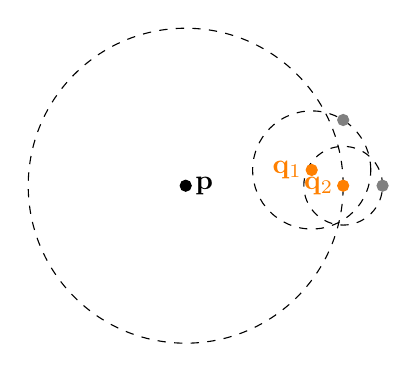
\begin{tikzpicture}
\filldraw[black] (0,0) circle (2pt) node[anchor=west] {$\mathbf{p}$};
\draw[dashed] (0,0) circle (2);
\draw[dashed] (2,0) circle (0.5);
\draw[dashed] (1.6,0.2) circle (0.75);
\filldraw[gray] (2,0.834429) circle (2pt);
\filldraw[gray] (2.5,0) circle (2pt);
\filldraw[orange] (1.6,0.2) circle (2pt) node[anchor=east] {$\mathbf{q}_1$};
\filldraw[orange] (2,0) circle (2pt) node[anchor=east] {$\mathbf{q}_2$};
\end{tikzpicture}
\caption{For $k=2$, $\mathbf{p}$ is an outlier as it has lower density than its neighbours.}
\label{lofoutlier}
\end{figure}
\noindent LOF is able to identify \textbf{local outliers}, but selecting a threshold beyond which a point is considered an outlier is difficult. \newl LOF introduces the idea of a \textbf{reachability distance}, which improves the stability of results within clusters/regions: within a local $k-$region around $\mathbf{p}$, it is simply the maximal distance to its $k-$neighbours; outside of that region, it is the actual distance from $\mathbf{p}$. 
\par In Figure \ref{reachability} (with $k=3$), for instance, the points $\mathbf{q}_1, \mathbf{q}_2, \mathbf{q}_3$ all have the same reachability distance from $\mathbf{p}$ as they are all $3$-neighbours of $\mathbf{p}$, that is, 
$$
d_{\text{reach}}(\mathbf{p}, \mathbf{q}_1) 
= d_{\text{reach}}(\mathbf{p}, \mathbf{q}_2)
= d_{\text{reach}}(\mathbf{p}, \mathbf{q}_3)
= d(\mathbf{p}, \mathbf{q}_3)
.$$
The point $\mathbf{q}_4$, on the other hand, has 
$d_{\text{reach}}(\mathbf{p}, \mathbf{q}_4)
= d(\mathbf{p}, \mathbf{q}_4)
$
as it is not a $k$-neighbour of $\mathbf{p}$.

\begin{figure}[H]
\hrule \vspace{0.4cm} \centering
\begin{tikzpicture}[x=0.96cm,y=0.96cm]
\filldraw[black] (0,0) circle (2pt) node[anchor=west] {$\mathbf{p}$};
\filldraw[black] (1,0) circle (2pt) node[anchor=west] {$\mathbf{q}_1$};
\filldraw[black] (1,-1) circle (2pt) node[anchor=west] {$\mathbf{q}_2$};
\filldraw[black] (0,2) circle (2pt) node[anchor=north] {$\mathbf{q}_3$};
\filldraw[black] (2,2) circle (2pt) node[anchor=west] {$\mathbf{q}_4$};
\draw[dashed] (0,0) circle (2);
\end{tikzpicture}
\caption{The region of uniform reachability distance around $\mathbf{p}$ for $k=3$.}
\label{reachability}
\end{figure}
\newpage\noindent  

\subsubsection*{DBSCAN}
Density-Based Spatial Clustering of Applications with Noise (DBSCAN) was proposed in 1996 by \cite{DBSCAN} 
(a summary can be found in Section 4.1.5 of \cite{A10}). 
As its name suggests, it is a density-based clustering algorithm that groups nearby points together and labels points that do not fall in the clusters as \textbf{anomalies}.

Hierarchical DBSCAN (HDBSCAN) \cite{HDBSCAN} was introduced in 2013.
It notably removes the problem of choosing the parameter for the radius of a neighbourhood by considering all possible radii. 
Further documentation can be found at \cite{HDBSCAN_code}. \newl 
In DBSCAN, 
\begin{itemize}[noitemsep]
\item a point $\mathbf{p}$ is a \textbf{core point} if there is a minimum of $m$ points within distance $r$ of $\mathbf{p}$;
\item a point $\mathbf{q}$ is a \textbf{border point} if it is not itself a core point but is within distance $r$ of one, and 
\item a point $\mathbf{o}$ is an \textbf{outlier} if it is neither a core nor a border point.
\end{itemize}
\begin{algorithm}[h]
\SetAlgoLined
\textbf{Input:} dataset $D$,
distance function $d$,
neighbourhood radius $r>0$,
minimum number of points to be considered a cluster $m\in\mathbb{N}$
\\$\textit{Clusters} = \{\}$
\\$\textit{Outliers} = \{\}$
\\\For{$\mathbf{p} \in D$}{
\If{$\mathbf{p} \in \textrm{Outliers} \cup \left( \cup_{C \in \textit{Clusters}} C \right)$}{
\textbf{continue}
}
Set $N(\mathbf{p}) = \{ \mathbf{q} \in D : d(\mathbf{p},\mathbf{q}) \leq r \}$
\\\If{$|N(\mathbf{p})| < m$}{
Add $\mathbf{p}$ to $\textit{Outliers}$
\\\textbf{continue}
}
\Else{
$\textit{Cluster} = N(\mathbf{p})$
\\\For{$\mathbf{q} \in \text{Cluster} \setminus \{\mathbf{p}\}$}{
\If{$\mathbf{q} \in \textit{Outliers}$}{
Remove $q$ from $\textit{Outliers}$
}
\ElseIf{$\mathbf{q} \in \cup_{C \in \textit{Clusters}} C$}{
\textbf{continue}
}
Set $N(\mathbf{q}) = \{ q' \in D : d(q,q') \leq r \}$
\\\If{$|N(\mathbf{q})| \geq m$}{
$\text{Cluster} = \text{Cluster} \cup N(\mathbf{q})$
}
}
}
Add $\textit{Cluster}$ to $\textit{Clusters}$
}
return $\textit{Outliers}$
\\\textbf{Output:} a list of \textit{outliers}
\caption{DBSCAN}
\label{dbscan}
\end{algorithm}







\begin{figure}[b]
\hrule \vspace{0.4cm}
\centering
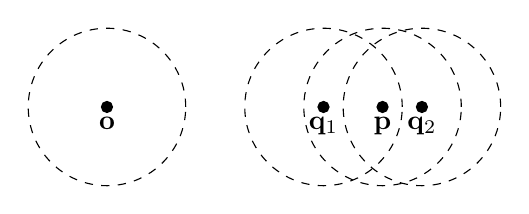
\begin{tikzpicture}
\filldraw[black] (-3.5,0) circle (2pt) node[anchor=north] {$\mathbf{o}$};
\draw[dashed] (-3.5,0) circle (1);
\filldraw[black] (0,0) circle (2pt) node[anchor=north] {$\mathbf{p}$};
\draw[dashed] (0,0) circle (1);
\filldraw[black] (-0.75,0) circle (2pt) node[anchor=north] {$\mathbf{q}_1$};
\draw[dashed] (-0.75,0) circle (1);
\filldraw[black] (0.5,0) circle (2pt) node[anchor=north] {$\mathbf{q}_2$};
\draw[dashed] (0.5,0) circle (1);
\end{tikzpicture}
\caption{For minimum neighbourhood size $m=2$ and this fixed radius $r$, $\mathbf{o}$ is an outlier, $\mathbf{p}$ a core point, and $\mathbf{q}_1$ and $\mathbf{q}_2$ are border points.}
\label{DBSCANlabels}
\end{figure}
\noindent DBSCAN considers each point in the dataset individually. If that point is an outlier, then it is added to a list of outliers. Otherwise if it is a core point, then its $r$-neighbourhood forms the beginning of a new cluster. Each point in this $r$-neighbourhood is then considered in turn, with the $r$-neighbourhoods of other core points contained in the neighbourhood being added to the cluster. \par This expansion repeats until all points have been examined. During this step points that were previously labelled as outliers may be updated as they become border points in this new cluster. This process continues until every point has either been assigned to a cluster or labelled as an outlier (see Algorithm~\ref{dbscan} and Figure~\ref{DBSCANlabels}).

While DBSCAN's dual use as a clustering algorithm may seem irrelevant in the outlier detection setting,
its ability to succesfully identify clusters is crucial to being able to label the remaining points as outliers.
\newl 
On the one hand, in DBSCAN the number of clusters does not need to be known beforehand (unlike in $k-$means and other clustering algorithms) and clusters of arbitrary shape can be detected. \par Furthermore, when using HDBSCAN, only the parameter for the minimum cluster size $m$ is required, which can be set fairly intuitively, which is not the case for the parameters in general clustering algorithms: if the elements of $D$ are $n-$dimensional, take $m\geq n+1$ (larger values of $m$ allow for better noise identification).
\newl On the other hand, DBSCAN is not deterministic, as border points can be assigned to different clusters depending on the order in which core points are considered (this does not affect its use as an anomaly detection algorithm, however).
\par In high dimensions, the ability of any distance function based on Euclidean distance to distinguish near and distant points diminishes due to the \textbf{Curse of Dimensionality}; thus in high dimension spaces, it  become ineffective (as do  other clustering algorithms). \par  Finally, DBSCAN cannot handle differences in local densities as the radius of a neighbourhood $r$ is fixed; this could lead to sparser clusters being labelled as outliers, or to outliers surrounding a denser cluster being included in the cluster.
This issue is overcome in HDBSCAN.

\subsubsection*{Isolation Forest}
The previously discussed approaches first construct models of what normal points look like, and then identify points that do not fit this model.
The Isolation Forest algorithm \cite{A15} introduced in 2008 instead tries to explicitly identify outliers under the assumptions that there are few outliers and that these outliers have very different attributes compared to normal points. Doing so allows the use of sampling techniques that increase algorithmic speed while decreasing memory requirements.
\begin{figure}[b]
\hrule \vspace{0.4cm}\centering
\begin{tikzpicture}[x=0.6cm,y=0.6cm]
\filldraw[black] (0,0) circle (2pt);
\filldraw[black] (4,2) circle (2pt);
\filldraw[black] (4.5,-2) circle (2pt);
\filldraw[black] (5,1) circle (2pt);
\draw[dashed] (0,2) -- (0,-2);
\draw[dashed] (5,2) -- (5,-2);
\draw[dashed] (0,2) -- (5,2);
\draw[dashed] (0,-2) -- (5,-2);
\draw (2,2) -- (2,-2);
\draw (2,-1) -- (5,-1);
\draw (4.25,2) -- (4.25,-1);
\end{tikzpicture}
\caption{A partitioning constructed during Isolation Tree generation.}
\label{isolationtree}
\end{figure}

The Isolation Forest algorithm tries to isolate anomalous points. It does this by randomly selecting an attribute and then randomly selecting a split value between that attribute's min and max values. This recursively partitions the points until every point is isolated in its own partition.
\newl Recursive partitioning yields a binary tree called an \textbf{Isolation Tree}. The root of this tree is the entire dataset; each node is a subset of the observations, and each branch corresponds to one of the generated partitions. The leaf nodes are singleton sets containing a single isolated point. Each point is then assigned a score derived from how deep in the tree its singleton partition appears (see Figure~\ref{isolationtree} and Algorithm~\ref{iTree}). 
\par As points that are shallower in the tree were easier to separate from the rest, these are the likely \textbf{outliers}. Since only shallow points are of interest, once the height of the tree has reached a given threshold (the expected height of a random binary tree, say), further construction of the tree can be stopped to decrease computational cost. \par 
Additionally, instead of building a tree from the entire dataset, a tree can be constructed from a subset. The location of any point within this smaller tree can then be estimated, again saving computational and memory resources. These two improvements are detailed in the original paper \cite{A15}. 
\newl Once a number of Isolation Trees have been randomly generated (\textbf{Isolation Forest}), a score can be computed for each point. This is done by searching each tree for the location of a given point and noting the path length required to reach it. Once a point's path length in each tree has been computed, the average path length is taken to be its score.
\newpage\noindent  It 
\begin{algorithm}[t]
\SetAlgoLined
\textbf{Input:} dataset $D$ % , integer $e$ current tree height, integer $\ell$ max tree height
\\\If{$|D| \leq 1$}{ % $e \geq \ell$ \textbf{or} 
return $\{\}$
}
\Else{
Let $\overline{A}$ be a list of attributes in $D$
\\Randomly select an attribute $A \in \overline{A}$
\\Randomly sample a point $s$ from $[\min_{\mathbf{q} \in D} A(\mathbf{q}), \max_{\mathbf{q} \in D} A(\mathbf{q})]$
\\Return 
$\text{Node}\begin{cases}
\text{LeftChild} &= \text{iTree}(\{\mathbf{q} \in D : A(\mathbf{q}) \leq s\}) % , e+1, \ell\})
\\\text{RightChild} &= \text{iTree}(\{\mathbf{q} \in D : A(\mathbf{q}) > s\}) % , e+1, \ell\})
\\\text{NodeValue} &= D
\end{cases}$
}
\textbf{Output:} Binary tree with node values that are subsets of $D$ % of height $\leq \ell - e$ 
\caption{Recursive Isolation Tree Construction: $\text{iTree}(D)$} % , e, \ell)$
\label{iTree}
\end{algorithm}
can 
\begin{algorithm}[h]
\SetAlgoLined
\textbf{Input:} dataset $D$, integer $t$ number of Isolation Trees % , integer $n$ subsampling size
\\\textit{Forest} = \{\}
% \\Set max tree height 
% $\ell = \lceil \log_2(n) \rceil$
\\\For{$i=1$ to $t$}{
% \\$D' \leftarrow sample(D, n)$
\textit{Tree} = $\text{iTree}(D)$ % , 0, \ell)$
\\Add \textit{Tree} to \textit{Forest}
}
\For{$\mathbf{p} \in D$}{
$\textit{PathLengths} = \{\}$
\\\For{\textit{Tree} in \textit{Forest}}{
% \\\If{$\{\mathbf{p}\}$ not a node of Tree}{
% }
% \\\Else{
Find the path length $\ell$ from the root of Tree to node $\{\mathbf{p}\}$
\\Add $\ell$ to $\textit{PathLengths}$
}
$\textit{AveragePathLength} = \frac{\sum_{\ell \in \textit{PathLengths}} \ell}{t}$
\\Set $a(\mathbf{p}) = 2^{- \frac{\textit{AveragePathLength}}{c(|D|)}} $
}
\textbf{Output:} Anomaly score $a(\mathbf{p}) \in [0,1]$ for each $\mathbf{p} \in D$
\caption{Isolation Forest}
\label{iForest}
\end{algorithm}
be desirable to construct a normalized anomaly score that is independent of the size of the dataset.
In order to do this, the expected path length of a random point in an Isolation Tree (i.e. binary tree) must be estimated. With $n = |D|$, it can be shown that the expected length is 
$$
c(n) 
= 2 H(n-1) - \frac{2(n-1)}{n},
$$
where $H(n-1)$ is the $(n-1)^{\text{th}}$ harmonic number, which can be approximated by $\ln(n-1) + 0.577$;
$c(n)$ is then used to normalize the final anomaly score $a(\mathbf{p})$ for $\mathbf{p} \in D$, which is given by
$$
\log_2 a(\mathbf{p})
= -\frac{\text{average path length to $\mathbf{p}$ in the Isolation Trees}}{c(n)}.
$$
Thus defined, $a(\mathbf{p})\in [0,1]$, with $a(\mathbf{p}) \approx 1$ suggesting $\mathbf{p}$ is an \textbf{anomaly}, $a(\mathbf{p}) \leq 0.5$ suggesting $\mathbf{p}$ is a normal point;
if all points receive a score around $0.5$, this suggests that there are no anomalies present.
\newl Isolation Forests have small time and memory requirements; can handle high dimensional data, and do not need observations to have been labeled anomalies in the training set, but the anomaly score assigned to a given point can have high variance over multiple runs of the algorithm. The authors of \cite{EIF} propose some solutions.
\begin{center}\rule{0.5\linewidth}{.4pt}\end{center}
In general, \text{density-based} schemes are more powerful than distance-based schemes when a dataset contains patterns with diverse characteristics, but less effective when the patterns are of comparable densities with the outliers \cite{JZ}.

